\documentclass[10pt,twocolumn,letterpaper]{article}
\usepackage[margin=.75in]{geometry}
\usepackage[T1]{fontenc}
\usepackage{courier}
\usepackage{newtxtext,amsmath,amssymb,graphicx,booktabs,natbib}
\usepackage[hyphens]{url}
\sloppy
\title{Why Oracle Recoverability Did Not Become a Practical Planning Gain}
\author{}\date{}
\begin{document}\maketitle
\begin{abstract}We analyze a failed transfer from answer-key diagnostic potential to evidence-only financial planning. On 96 TAT-QA contexts, a planner changes correct delivery 6 to 10 and wrong delivery 23 to 25, while correct candidates decrease 26 to 25. It fails its prespecified practical requirement; a secondary 28-context comparison gives no delivery gain. We place these findings alongside a complementary resident-team deployment comparison, stronger baselines, scoring sensitivity and resource limits. Complete historical and statistical support is retained separately.\end{abstract}

\section{Question and Scope}
Can an evidence-only planner realize the recovery suggested by answer-key diagnostic interventions? We examine this question in completed financial program-generation experiments. Our contribution is a failure analysis of specific local recipes, not a new winning algorithm. Financial programs can execute correctly while selecting the wrong period, row, unit or operation. A verifier can also reduce wrong delivery by withholding most answers. Candidate construction and delivered correctness must therefore remain distinct.

\section{Design and Measurements}
The planning comparison uses four completed arms on 96 project-held-out TAT-QA contexts: direct 7B, program-generating 7B, a smaller multi-role pipeline (MAS), and planner MAS. Models belong to Qwen2.5; the full record specifies model hashes, adapters, prompts and decoding \citep{qwen}. Evidence packets do not expose answer labels. Programs refer to source quantities and arithmetic steps; deterministic execution establishes arithmetic/provenance constraints, not financial semantic validity. The planner predicts operations, dependencies and VALUE placeholders from question/evidence without answer-key supervision. Its token allocation also changes the actor budget, so this is a pipeline intervention rather than an isolated planning-stage causal effect.

Let $K_i$ indicate a correct executable candidate and $D_i$ delivery. Correct delivery is $n^{-1}\sum_i K_iD_i$; wrong delivery is $n^{-1}\sum_i(1-K_i)D_i$. Withholding is $n^{-1}\sum_i(1-D_i)$. These observables distinguish generation from acceptance \citep{selective}. The prespecified practical requirement combines a positive paired correct-delivery interval with no observed increase in wrong delivery. A secondary 28-context cohort tests the direction again.

The Windows experiment is a nominal 8 GB \emph{application-budget tier} on a 16.39 GB host. A 6.1 GB worker commit ceiling and sampled working-set guard do not establish physical 8 GB feasibility or absence of paging. Greedy single-seed runs do not measure training/decoding variation. FinQA and arithmetic TAT-QA are public financial reasoning benchmarks \citep{finqa,tatqa}; project-held-out filtering does not exclude pretraining contamination.

\section{Results: Recovery Does Not Establish Improvement}
\begin{table}[t]\centering\small
\caption{All primary planner arms, $n=96$. C/W/H are correct delivered, wrong delivered and withheld.}\label{tab:planner}
\begin{tabular}{lrrr}\toprule Recipe&C&W&H\\\midrule Direct 7B&19&76&1\\Program 7B&15&80&1\\MAS&6&23&67\\Planner MAS&10&25&61\\\bottomrule\end{tabular}\end{table}
The planner gains four correct deliveries and loses none, but adds two wrong deliveries (Table~\ref{tab:planner}). The correct-delivery change is $+4.2$ percentage points, with paired context-bootstrap 95\% interval approximately $[+1.0,+8.3]$; exact paired $p=0.125$. Sparse discordant pairs and the bootstrap/exact-test disagreement preclude an established accuracy improvement. More importantly, the practical conjunction fails because wrong delivery increases. Correct executable candidates decrease from 26 to 25: the delivered gain is not a net generation gain.

On the secondary 28-context cohort both MAS arms deliver 2 correct, 10 wrong and withhold 16; correct candidates decrease 5 to 3. The attempted 7B comparison stops after a two-context prefix because of allocation failure, leaving that baseline incomplete. Planner median resident request time rises 25.2 to 33.9 seconds; generated tokens rise 6672 to 9863. Commit remains about 5.26 GB. Cross-arm direct/program timings include model loading and are not matched resident-latency comparisons.

The oracle diagnostic supplies reference operation structure and an operand shortlist on 15 enriched FinQA cases. Official execution matches change 0/0/4/10 across neither/operands/structure/both. These answer-key inputs supply unavailable solution information and are neither a deployable planner nor a universal reasoning upper bound. Even the combined intervention yields only 7 reported-answer matches; numerical scoring conventions are not interchangeable.

\begin{figure*}[t]\centering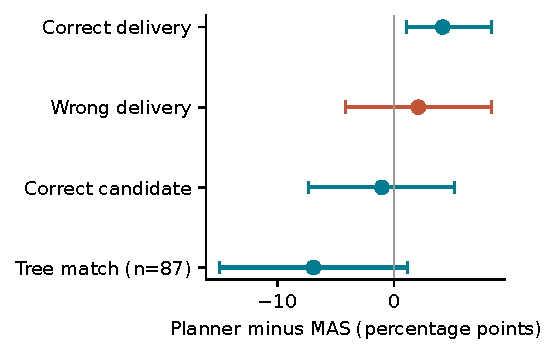
\includegraphics[width=.60\textwidth]{figures/planner_effects.pdf}\caption{Planner-minus-MAS changes with paired context-bootstrap 95\% intervals. Sparse exact-test evidence and the no-wrong-increase criterion remain essential.}\end{figure*}\section{Complementary Deployment Evidence}
A separate nominal 16 GB deployment study compares a quantized 14B recipe with a resident 1.5B/3B/0.5B F16 team on 160 FinQA questions from 50 reports. Reported C/W/H is 78/48/34 versus 5/3/152; raw execution matching is 38/88/34 versus 5/3/152. The team produces only 10 executable candidates and 150 INSUFFICIENT drafts. All annotated evidence spans are present in 138 packets; the team still delivers only 5 correct there versus 74 for the larger recipe. This rules out missing annotated spans as the sole descriptive explanation, not model/prompt confounding.

The completed Ubuntu replication preserves the recorded outcomes. Across 668817 memory samples and 16 attempts, sampled process swap is zero and peak application RSS is 10.946 GB below the 11.5 GB guard. Interruptions and missing original export/log artifacts prevent an uninterrupted-deployment claim. Windows commit and Linux RSS/swap evidence are different measurements, not a cross-tier causal scaling curve.

Other observations prevent a one-sided interpretation. Direct 7B outperforms direct 3B on 120 fresh TAT-QA contexts 29 versus 12 ($p=0.00151$), but direct-versus-program effects depend on task/scorer. Matched Q4/Q8 FinQA conditions each achieve 2/96 official matches, with two gains and two losses. Retrieval expansion and repair do not supply a robust practical gain; critic-pilot advantages fail transfer criteria. Disabling prompt caching preserves fixed-workload predictions while reducing peak worker commit approximately 6.101 to 5.264 GB, an engineering improvement rather than a reasoning gain. Complete overlapping historical cohorts and all adverse/null outcomes remain in the supplement.

\section{Relation to Prior Work and Limitations}
Program-aided methods separate generation from execution \citep{pal,pot}; that separation does not solve semantic binding. Equal-thinking-budget comparisons and broader multiagent failure taxonomies already question simple collaboration advantages \citep{equalbudget,mast}. We do not claim novelty for decomposition, verification or resource-aware evaluation, and do not reproduce every published baseline.

Generality remains limited by one model family, selected prompts/grammar, public financial subsets and recipe confounding. Report/company clustering is available for FinQA but report mapping is unavailable for TAT-QA. Enriched oracle cases and overlapping development cohorts are exploratory, not independent replications. Numerical benchmark agreement is not expert financial adjudication or operational safety. The full supplement retains paired uncertainty, scorer sensitivity, conditional mathematical assumptions, historical baselines and worked failures.

\section{Conclusion}
The planner fails its practical criterion. Four additional correct deliveries do not establish a generation gain when correct candidates decrease and wrong delivery increases. Oracle recoverability and deployable improvement must remain distinct.
\section*{Support and AI Assistance}
The accompanying 29-page audited supplement preserves complete methods, all cohorts, historical outcomes, statistical derivations and examples. Codex assisted this adaptation and code-based checks of preserved evidence; no new inference was run. Human authors must review correctness, originality, declarations and destination-specific rules before submission. This generic draft is not certified for any named workshop.
\bibliographystyle{plainnat}\bibliography{references}
\end{document}
